% 原书印刷269中--276中／PDF物理293中--300中.
\subsection{位移凸性}\label{sec:7.3}
上一节关于凸性的全部讨论中，总是考虑标准凸插值$[0,1]\ni t\mapsto(1-t)\mu_0+t\mu_1$. 不过，另一种与空间$\mathbb W_p(\Omega)$的度量结构更紧密相关的凸性概念，也可能有用.

先给出一般定义.
\begin{definition}\label{obj:7.23}\index{D042@位移凸性（displacement convexity）|hyperpage}
在测地度量空间$X$中，若对每两个点$x_0,x_1\in X$，都存在连接$\omega(0)=x_0$与$\omega(1)=x_1$的常速测地线$\omega$，使$[0,1]\ni t\mapsto F(\omega(t))$为凸，则称$F:X\to\mathbb R\cup\{+\infty\}$测地凸.
\end{definition}
在$\mathbb R^d$或任何其他以线段为唯一测地线的赋范向量空间中，这显然化为通常的凸性（注意，在任意赋范向量空间中线段都是测地线，但未必是唯一的测地线，例如$L^1$、$L^\infty$或任何非严格凸空间）. 顺便说，在测地线不唯一的空间中，上述定义可能引起讨论，因为也可以选择将沿每条测地线$\omega$都满足测地不等式的泛函定义为测地凸. 但这里给出的定义是通常采用的，因为它还满足一些稳定性结果，而要求每条测地线上都凸的更强定义不具备这些结果.

空间$\mathbb W_p(\Omega)$中的测地凸性概念由McCann在\cite{b229}中引入；由于我们知道如何刻画这一空间中的测地线，它尤其有意义. 这种凸性通常称为位移凸性. 注意，它先验地可能依赖于指数$p$.

\subsubsection[势能与相互作用能的位移凸性]{$\mathscr V$与$\mathscr W$的位移凸性}\label{sec:7.3.1}
\phantomsection\label{idx:i43-p270}\index{D043@位移插值（displacement interpolation）|hyperpage}
\phantomsection\label{idx:i66-p270}\index{G065@测地线（geodesics）!066@$\mathbb W_p$中（in $\mathbb W_p$）|hyperpage}
回顾，距离$W_p$的测地线形如$\mu_t=(\pi_t)_\#\gamma$，其中$\gamma$是成本$c(x,y)=|x-y|^p$的最优运输，且$\pi_t(x,y)=(1-t)x+ty$.
\begin{proposition}\label{obj:7.24}\index{I079@相互作用能（interaction energy）|hyperpage}\index{P116@势能（potential energy）|hyperpage}
泛函$\mathscr V$位移凸，当且仅当$V$为凸. 若$W$为凸，则泛函$\mathscr W$位移凸.
\end{proposition}
\begin{proof}
先考虑$\mathscr V$，假设$V$凸. 计算$\mathscr V(\mu_t)$：
\[
 \mathscr V(\mu_t)=\int V\,d(\pi_t)_\#\gamma
                 =\int V((1-t)x+ty)\,d\gamma.
\]
由这一公式显然可见，若$V$凸，则$t\mapsto\mathscr V(\mu_t)$凸.

另一方面，$V$的凸性是$\mathscr V$凸的必要条件，只需考虑形如$\mu_t=\delta_{(1-t)x+ty}$的测地线便容易验证，因为$\mathscr V(\mu_t)=V((1-t)x+ty)$.

$\mathscr W$凸性的证明类似：考虑
\[
\begin{aligned}
 \mathscr W(\mu_t)&=\int W(x,x')\,d(\pi_t)_\#\gamma(x)\,d(\pi_t)_\#\gamma(x')\\
 &=\int W((1-t)x+ty,(1-t)x'+ty')\,d\gamma(x,y)\,d\gamma(x',y'),
\end{aligned}
\]
由此容易得到凸性的条件.
\end{proof}
注意，没有声称$W$的凸性是$\mathscr W$凸的必要条件，因为一般并非如此. 例如，考虑如下的一维情形.
\begin{proposition}\label{obj:7.25}
设$\Omega=(a,b)$、$\Delta^+=\{(x,y)\in\Omega\times\Omega:y\geq x\}$、$\Delta^-=\{(x,y)\in\Omega\times\Omega:y\leq x\}$. 则只需$W$限制在$\Delta^+$与$\Delta^-$上时为凸，就能得到$\mathscr W$的位移凸性.
\end{proposition}
\begin{proof}
只需考虑\autoref{obj:7.24}的证明，并验证对$(x,y),(x',y')\in\operatorname{spt}(\gamma)$，所有线段$t\mapsto((1-t)x+ty,(1-t)x'+ty')$都包含在$\Delta^+$或$\Delta^-$中. 这由\autoref{sec:2.2}中证明的$\operatorname{spt}(\gamma)$的单调性保证. 事实上，已经证明对每个严格凸成本，（唯一的）最优运输方案$\gamma$满足
\[
 (x,y),(x',y')\in\operatorname{spt}(\gamma),\quad x<x'
                      \quad\Longrightarrow\quad y\leq y'.
\]
这意味着若$x<x'$，则$(x,x')\in\Delta^+$与$(y,y')\in\Delta^+$，由凸性，$((1-t)x+ty,(1-t)x'+ty')\in\Delta^+$. 类似地，对$x>x'$，得到线段包含在$\Delta^-$中. 若$x=x'$，只需从$y$的角度看运输方案，得到蕴含$y<y'\Longrightarrow x\leq x'$，并以同样方式得出结论. 唯一单独留下的情形是$x=x'$且$y=y'$，但此时线段化为一个点.

这证明了$\mathscr W$沿$\mathbb W_p$中测地线的凸性，其中$p>1$. 若选取同一个$\gamma$作为最优运输方案，它对$W_1$也适用（此时最优方案不唯一，但这已足以构造一条使泛函凸的测地线）.
\end{proof}
这一判据的一个有趣推论是，对$\mathscr X=H^1([-1,1])$，对偶范数平方$\mu\mapsto\|\mu\|_{\mathscr X'}^2$实际上位移凸，这是\autoref{obj:7.6}的刻画的推论（但对$\mathscr X=H_0^1$不适用）. 文献\cite{b62,b110}指出并使用了这一点.

这是一个在某种意义上涉及导数的位移凸泛函的例子. 可以说，作为$H^{-1}$范数，它是一个$-1$阶泛函. 非零阶的位移凸泛函并不常见. 对一阶情形，唯一已知例子见\cite{b115}，而且仍然只在一维可用. 多维情形尚无已知结果.

\subsubsection[密度泛函的位移凸性]{$\mathscr F$的位移凸性}\label{sec:7.3.2}
最有意义的位移凸性结果涉及依赖密度的泛函.

为考察这些泛函，需要一些技术性事实.

起点是像测度密度的计算，通过标准换元技巧完成，正如备忘\autoref{box:1.14}中所见.

随后，强调一个有趣的计算.
\begin{lemma}\label{obj:7.26}
设$A$为$d\times d$矩阵，其特征值$\lambda_i$均为实数且大于$-1$（例如，$A$对称且$\mathrm I+A\geq0$时就是如此）. 则$[0,1]\ni t\mapsto g(t):=\det(\mathrm I+tA)^{1/d}$为凹.
\end{lemma}
\begin{proof}
可以在适当的基下将$A$写成三角矩阵，得到
\[
 g(t)^d=\prod_{i=1}^d(1+t\lambda_i).
\]
求导，
\[
 dg(t)^{d-1}g'(t)=\sum_{j=1}^d\lambda_j
           \prod_{i=1,\,i\ne j}^d(1+t\lambda_i)
         =g(t)^d\sum_{j=1}^d\frac{\lambda_j}{1+t\lambda_j},
\]
即$dg'(t)=g(t)\sum_{j=1}^d\frac{\lambda_j}{1+t\lambda_j}$. 再求一次导数，得到
\[
 dg''(t)=g'(t)\sum_{j=1}^d\frac{\lambda_j}{1+t\lambda_j}
       -g(t)\sum_{j=1}^d\frac{\lambda_j^2}{(1+t\lambda_j)^2}.
\]
此处使用平方平均与算术平均不等式，给出
\[
 \sum_{j=1}^d\frac{\lambda_j^2}{(1+t\lambda_j)^2}
 \geq\frac1d\left(\sum_{j=1}^d\frac{\lambda_j}{1+t\lambda_j}\right)^2
 =d\left(\frac{g'(t)}{g(t)}\right)^2,
\]
从而
\[
 dg''(t)\leq d\frac{g'(t)^2}{g(t)}-d\frac{g'(t)^2}{g(t)}=0,
\]
这证明了$g$的凹性.
\end{proof}
\begin{remark}\label{obj:7.27}
注意，在维数$d=1$时，上述引理显然成立，而且$g$实际上是仿射的.
\end{remark}
现在可以陈述主要定理，它是\cite{b229}的主要结果.
\begin{theorem}\label{obj:7.28}
假设$f$凸且超线性，$f(0)=0$，并且$s\mapsto s^{-d}f(s^d)$凸且递减. 假设$\Omega$凸，取$1<p<\infty$. 则$\mathscr F$在$\mathbb W_p$中测地凸.
\end{theorem}
\begin{proof}
考虑满足$\mathscr F(\mu_0),\mathscr F(\mu_1)<+\infty$的两个测度$\mu_0,\mu_1$. 它们绝对连续，因而二者之间存在唯一的常速测地线$\mu_t$（见\autoref{obj:5.27}与\autoref{obj:5.32}），其形式为$\mu_t=(\mathrm T_t)_\#\mu_0$，其中$\mathrm T_t=\mathrm{id}+t(\mathrm T-\mathrm{id})$. 注意，由\autoref{obj:4.23}，$\mathrm T_t$单射.

\phantomsection\label{idx:i30-p272}\index{C030@可数Lipschitz（countably Lipschitz）|hyperpage}
先看较容易的$p=2$情形. 此时$\mathrm T_t(x)=x-t\nabla\varphi(x)$，其中$\frac{x^2}2-\varphi$为凸. 由\autoref{obj:3.16}，这意味着$\nabla\varphi$可数Lipschitz，$\mathrm T_t$也如此. 因此它们几乎处处近似可微\footnote{事实上，还知道$D^2\varphi$几乎处处存在：凸函数几乎处处二次可微（例如见\cite{b160}，原始结果发表于\cite{b6}）.}. Hessian矩阵$D^2\varphi$（等价地，$\nabla\phi$的近似梯度）对称，且$D^2\varphi\leq\mathrm I$. 定义$A(x)=-D^2\varphi(x)$. \phantomsection\label{idx:i39-p273}\index{D039@Jacobi行列式（determinant of the Jacobian）|hyperpage}
由像测度的密度公式，已知$\mu_t$绝对连续，可将其密度$\varrho_t$写成$\varrho_t(y)=\varrho(\mathrm T_t^{-1}(y))/\det(\mathrm I+tA(\mathrm T_t^{-1}(y)))$，从而
\[
\begin{aligned}
 \mathscr F(\mu_t)&=\int f\left(\frac{\varrho(\mathrm T_t^{-1}(y))}
             {\det(\mathrm I+tA(\mathrm T_t^{-1}(y)))}\right)\,dy\\
 &=\int f\left(\frac{\varrho(x)}{\det(\mathrm I+tA(x))}\right)
                  \det(\mathrm I+tA(x))\,dx,
\end{aligned}
\]
这里使用换元$x=\mathrm T_t^{-1}(y)$，得到$y=\mathrm T_t(x)$及$dy=\det D\mathrm T_t(x)\,dx=\det(\mathrm I+tA(x))\,dx$.

由\autoref{obj:7.26}，已知$\det(\mathrm I+tA(x))=g(t,x)^d$，其中函数$g:[0,1]\times\Omega$关于$t$为凹. 一个一般事实是，凸递减函数与凹函数复合，得到凸函数. 这意味着
\[
 t\mapsto f\left(\frac{\varrho(x)}{g(t,x)^d}\right)g(t,x)^d
\]
为凸（若$\varrho(x)\ne0$，使用了关于$f$的假设，以及$t\mapsto g(t,x)/\varrho(x)^{1/d}$为凹这一事实；若$\varrho(x)=0$，则该函数就是零）. 最后证明了$t\mapsto\mathscr F(\mu_t)$的凸性.

现在必须推广到$p\ne2$的情形. 此时，令$h(z)=\frac1p|z|^p$，有$\mathrm T_t(x)=x-t\nabla h^*(\nabla\varphi(x))$. 注意$h$与$h^*$均属于$C^2(\mathbb R^d\setminus\{0\})$. 首先注意，忽略零测集后，可以将$\Omega$分成两个可测部分：$\nabla\varphi=0$的集合$\Omega'$与$\nabla\varphi\ne0$的集合$\Omega''$. 所作分析与\autoref{sec:3.3.2}非常类似. 在$\Omega'$上，$\mathrm T$为恒等映射，$\mathrm T_t$也是恒等映射，$\mathrm T_t$同样如此. 由于$\mathrm T_t$单射，密度在这一集合上保持不变，可以取$A=0$应用\autoref{obj:7.26}. 相反，集合$\Omega''$可以分解为集合$\Omega_{ij}$的可数并，在这些集合中$x\in B_i$、$\mathrm T(x)\in B_j$，其中$(B_i)_i$是生成$\mathbb R^d$拓扑的一族可数球，并且只取满足$B_i\cap B_j=\varnothing$的配对. 在这一集合上，$\varphi=\psi^c$还与$\varphi_{ij}$相同，后者定义为函数$x\mapsto\inf_{y\in B_j}h(x-y)-\psi(y)$在$B_i$上的限制；它是$\lambda$凹的，其中$\lambda=\sup\{\|D^2h(z)\|:z\in B_j-B_i\}$. 这证明$\varphi_{ij}$具有与凹函数相同的正则性，且$\nabla\varphi$与$\nabla h^*(\nabla\varphi)$在$\Omega''$上可数Lipschitz. 特别地，$D^2\varphi$几乎处处存在.

固定$\Omega''$中$\nabla\varphi(x_0)$与$D^2\varphi(x_0)$都存在的点$x_0$，可写出$\varphi(x)\leq h(x-\mathrm T(x_0))-\psi(\mathrm T(x_0))$，这一不等式对所有$x$成立，且在$x=x_0$时取等号. 特别地，得到$D^2\varphi(x_0)\leq D^2h(x_0-\mathrm T(x_0))=D^2h(\nabla h^*(\nabla\varphi(x_0)))$. 由Legendre变换的一般性质，
\[
 D^2h(\nabla h^*(z))=[D^2h^*(z)]^{-1}
\]
（只需对关系$\nabla h(\nabla h^*(z))=z$求导）. 因而可以取$A(x)=-D^2h^*(\nabla\varphi(x))D^2\varphi(x)$应用\autoref{obj:7.26}，因为它可对角化，且特征值大于$-1$（见下方\autoref{box:7.2}）.
\end{proof}

\Needspace{8\baselineskip}
\begin{sourcebox}{备忘：对称矩阵乘积的对角化}\label{box:7.2}
众所周知，对称矩阵可在$\mathbb R$上对角化. 一个较微妙的结果如下：
\begin{theorem*}
若$A,B$是对称$d\times d$矩阵，且$A$正定，则$AB$可对角化.
\end{theorem*}
不证明这一结果，只证明下列较弱结果.
\begin{proposition*}
若$A,B$是对称$d\times d$矩阵，且$A$正定，则$AB$具有实特征值.
\end{proposition*}
\begin{proof}
假设$\lambda\in\mathbb C$是$AB$的特征值，即对某个向量$\mathbf v\in\mathbb C^n\setminus\{0\}$有$AB\mathbf v=\lambda\mathbf v$. 与$A^{-1}\mathbf v$取Hermite内积，即$\overline{\mathbf v}^{\,t}B\mathbf v=\lambda\overline{\mathbf v}^{\,t}A^{-1}\mathbf v$，其中上标$t$表示矩阵意义下的转置. 注意，分别将$B$与$A^{-1}$对角化可知，$\overline{\mathbf v}^{\,t}B\mathbf v$与$\overline{\mathbf v}^{\,t}A^{-1}\mathbf v$都是实数，且$\overline{\mathbf v}^{\,t}A^{-1}\mathbf v>0$. 因而$\lambda\in\mathbb R$.
\end{proof}
还需要另一个重要事实.
\begin{proposition*}
若$B\leq A^{-1}$（按对称矩阵的意义，即对所有$\mathbf v$有$\mathbf v^t(A^{-1}-B)\mathbf v\geq0$），则$AB$的全部特征值$\lambda_i$均满足$\lambda_i\leq1$.
\end{proposition*}
\begin{proof}
同样写出$AB\mathbf v=\lambda\mathbf v$，推得$\overline{\mathbf v}^{\,t}B\mathbf v=\lambda\overline{\mathbf v}^{\,t}A^{-1}\mathbf v$. 这意味着$\overline{\mathbf v}^{\,t}A^{-1}\mathbf v\geq\overline{\mathbf v}^{\,t}B\mathbf v=\lambda\overline{\mathbf v}^{\,t}A^{-1}\mathbf v$，因而$\lambda\leq1$.
\end{proof}
\end{sourcebox}

看几个满足\autoref{obj:7.28}假设的凸函数的简单例子. 例如：
\begin{itemize}
 \item 对任意$q>1$，函数$f(t)=t^q$满足这些假设，因为$s^df(s^{-d})=s^{-d(q-1)}$凸且递减；
 \item \phantomsection\label{idx:i51-p274}\index{E051@熵（entropy）|hyperpage}
熵函数$f(t)=t\log t$也满足这些假设，因为$s^df(s^{-d})=-d\log s$凸且递减；
 \item 若$1-\frac1d\leq m<1$，函数$f(t)=-t^m$为凸，计算$s^df(s^{-d})=-t^{m(1-d)}$，由于$m(1-d)<1$，得到凸递减函数；但这些函数缺少超线性假设，不过这并不妨碍将\autoref{obj:7.28}的同一证明用于先验地假定$\mu_0$、$\mu_1$绝对连续的情形.
\end{itemize}
下面看\autoref{obj:7.28}在$f(t)=t^q$、$q>1$时的一些推论.
\begin{proposition}\label{obj:7.29}
考虑指数$1<q\leq+\infty$与两个概率测度$\mu_0,\mu_1\in L^q(\Omega)$（意思是它们绝对连续，且密度属于$L^q$）. 取连接它们的$\mathbb W_p$中的（唯一）测地线$\mu_t$，其中$p>1$. 则测度$\mu_t$也属于$L^q$，且$\|\mu_t\|_{L^q}\leq\max\{\|\mu_0\|_{L^q},\|\mu_1\|_{L^q}\}$. 当$q<+\infty$时，还有$\|\mu_t\|_{L^q}^q\leq(1-t)\|\mu_0\|_{L^q}^q+t\|\mu_1\|_{L^q}^q$.
\end{proposition}
\begin{proof}
$q<+\infty$的情形容易由\autoref{obj:7.28}得到. 事实上，若使用$f(t)=t^q$，有$\mathscr F(\mu)=\|\mu\|_{L^q}^q$. 因而
\[
 \|\mu_t\|_{L^q}^q\leq(1-t)\|\mu_0\|_{L^q}^q+t\|\mu_1\|_{L^q}^q
 \leq\bigl(\max\{\|\mu_0\|_{L^q},\|\mu_1\|_{L^q}\}\bigr)^q.
\]
由此得到所需$L^q$估计.

$q=+\infty$的情形，只需取$q$次方根，再令$q\to+\infty$.
\end{proof}

以一个观察结束本小节：在一维情形，还能说得更多.
\begin{proposition}\label{obj:7.30}\index{D042@位移凸性（displacement convexity）|hyperpage}
假设$d=1$、$\Omega=[a,b]\subset\mathbb R$，取$q>0$. 则对$\varrho\ll\mathscr L^1$由$F(\varrho)=\int_a^b\varrho(x)^{-q}\,dx$定义的泛函$F$在$\mathbb W_p(\Omega)$中位移凸. 特别地，若$\varrho_0,\varrho_1\geq c>0$，则对每个$t\in[0,1]$也有$\varrho_t(x)\geq c$，其中$\varrho_t$是连接$\varrho_0$与$\varrho_1$的测地线.
\end{proposition}
\begin{proof}
注意，函数$f(s)=s^{-q}$在$s>0$时为凸，且$s\mapsto s^df(s^{-d})=s^{q+1}$凸但递增. 不过，重读\autoref{obj:7.28}的证明可见，只是为了保证与$g$复合后为凸，才需要它递减；但这里$g$仿射，因此$s\mapsto s^df(s^{-d})$的凸性就足够. 此外，若假设$F(\varrho)<+\infty$，则$\varrho>0$几乎处处，表明无需假设$f(0)=0$. 这证明了所需的位移凸性. 为得到测地线上的下界，只需像\autoref{obj:7.29}中一样，令$q\to\infty$.
\end{proof}

\subsubsection{广义测地线上的凸性}\label{sec:7.3.3}\index{G064@广义测地线（generalized geodesics）|hyperpage}
令人失望的是，泛函$\mu\mapsto W_2^2(\mu,\nu)$一般并不位移凸. 这似乎违背直觉，因为距离平方通常是良好的凸函数. 不过，从下列简单例子可以看出失败之处. 取$\nu=\frac12\delta_{(1,0)}+\frac12\delta_{(-1,0)}$与$\mu_t=\frac12\delta_{(t,a)}+\frac12\delta_{(-t,-a)}$. 若$a>1$，曲线$\mu_t$就是$\mu_{-1}$与$\mu_1$之间的测地线（因为这些测度之间的最优运输将$(a,-1)$送到$(a,1)$，将$(-a,1)$送到$(-a,-1)$）. 但计算$W_2^2(\mu_t,\nu)$，得到
\[
 W_2^2(\mu_t,\nu)=a^2+(1-t)^2\wedge(1+t)^2.
\]
而这一函数并不凸！（见\autoref{fig:7.1}.）

\begin{figure}[htbp]
 \centering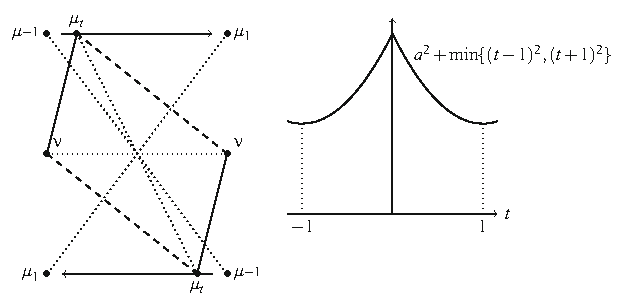
\includegraphics[width=.9\textwidth]{assets/ch07-fig7-1.pdf}
 \caption{距离$W_2^2(\mu_t,\nu)$.}
 \label{fig:7.1}
\end{figure}

这个简单泛函缺少测地凸性\footnote{顺便指出，甚至可以证明该泛函在某种意义上是测地凹的，如\cite{b15}的定理7.3.2所示.}，给许多问题带来困难（特别是通过EVI条件研究梯度流的某些度量方法；见\autoref{sec:8.4.1}），因而提出了另一种概念，即沿广义测地线的凸性.
\begin{definition}\label{obj:7.31}
固定绝对连续概率测度$\varrho\in\mathscr P(\Omega)$，对每对$\mu_0,\mu_1\in\mathscr P(\Omega)$，将曲线$\mu_t=((1-t)\mathrm T_0+t\mathrm T_1)_\#\varrho$称为$\mathbb W_2(\Omega)$中以$\varrho$为基的$\mu_0$与$\mu_1$之间的广义测地线，其中$\mathrm T_0$是从$\varrho$到$\mu_0$的最优运输映射（成本$|x-y|^2$），$\mathrm T_1$则从$\varrho$到$\mu_1$.
\end{definition}
显然，$t\mapsto W_2^2(\mu_t,\varrho)$满足
\[
\begin{aligned}
 W_2^2(\mu_t,\varrho)&\leq\int|((1-t)\mathrm T_0(x)+t\mathrm T_1(x))-x|^2\,d\varrho(x)\\
 &\leq(1-t)\int|\mathrm T_0(x)-x|^2\,d\varrho(x)
          +t\int|\mathrm T_1(x)-x|^2\,d\varrho(x)\\
 &=(1-t)W_2^2(\mu_0,\varrho)+tW_2^2(\mu_1,\varrho),
\end{aligned}
\]
因而得到所需的沿该曲线的凸性. 此外，与本节所作类似的考虑表明，已经证明为测地凸的所有泛函，也沿广义测地线为凸. 这里不展开这些证明，更多细节见\cite{b15}：对于泛函$\mathscr F$，须将\autoref{obj:7.26}改为“只要$A$与$B$对称正定，$t\mapsto\det((1-t)A+tB)^{1/d}$就为凹”（证明类似）.
